% =====================================================================
%  UR5e Safe Reinforcement Learning Grasping -- thesis book
%  Touhid  |  Dept. of Mechatronics Engineering, KUET
%
%  Build:  latexmk -pdf main.tex        (or the VS Code LaTeX Workshop button)
%  Engine: pdflatex + newtx  (Times New Roman metrics)
% =====================================================================

% ---------------------------------------------------------------------
%  >>> FONT SIZE SWITCH <<<  the only place the body size is set.
%  UNRESOLVED since Day 7: project instructions say 12pt, a personal note
%  says 14pt.  Change the number below and rebuild -- nothing else needs
%  to move.  (extbook is used instead of book precisely because the
%  standard classes cannot do 14pt.)
% ---------------------------------------------------------------------
\documentclass[12pt,a4paper,oneside]{extbook}

% ---------------------------------------------------------------------
%  Formatting.  Pass [final] instead of [draft] to hide all draft notes
%  and turn every unsourced \todocite into a hard build error.
%  Replace this line with the official KUET class when it arrives.
% ---------------------------------------------------------------------
\usepackage[draft]{thesis-format}

% Title exactly as filed (logbook/08_project_context.md).
\title{Safe Adaptive Image-Based Visual Servoing with Constrained Reinforcement
       Learning for Precision Grasping on a UR5 Manipulator:\\
       From Simulation to Real Hardware}
\author{Touhid}
\date{\today}

\begin{document}

% ---------------------------------------------------------------------
%  Front matter, in the order KUET requires
%  (logbook/08_project_context.md, "Required KUET thesis-book structure")
% ---------------------------------------------------------------------
\frontmatter
% Title page -- KUET_FORMAT_SPEC.md section 7.
% Wording below is the template's own boilerplate, copied verbatim.
% Note "fulfillment" is the template's spelling -- do not anglicise it.
\begin{titlepage}
\thispagestyle{empty}
\centering
\setstretch{1.25}\vspace*{-10mm}

{\fontsize{14}{20}\bfseries \thesistitle \par}

\vspace{2\baselineskip}

{\fontsize{12}{18}\selectfont A thesis submitted in partial fulfillment of the requirements for the degree of \par}
{\fontsize{12}{18}\selectfont Bachelor of Science \par}
{\fontsize{12}{18}\selectfont in \par}
{\fontsize{12}{18}\selectfont Mechatronics Engineering \par}

\vspace{0.5\baselineskip}
{\fontsize{12}{18}\selectfont by \par}
{\fontsize{12}{18}\bfseries \studentname \par}

\vspace{1.5\baselineskip}

{\fontsize{12}{18}\selectfont Supervised by \par}
{\fontsize{12}{18}\bfseries \supervisorname \par}

\vspace{1.5\baselineskip}

% University monogram. Drop the KUET crest in as figures/kuet_monogram.pdf
% (or .png) and it appears automatically; until then a labelled box holds
% the space so the layout does not shift when it arrives.
\IfFileExists{figures/kuet_monogram.pdf}%
  {
\includegraphics[height=28mm]{kuet_monogram.pdf}}%
  {\IfFileExists{figures/kuet_monogram.png}%
    {
\includegraphics[height=28mm]{kuet_monogram.png}}%
    {\framebox[30mm]{\rule{0pt}{28mm}\small\itshape monogram}}}

\vspace{\baselineskip}

{\fontsize{12}{18}\selectfont Department of Mechatronics Engineering \par}
{\fontsize{12}{18}\selectfont Khulna University of Engineering \& Technology \par}
{\fontsize{12}{18}\selectfont Khulna-9203, Bangladesh \par}

\vspace{0.5\baselineskip}

{\fontsize{12}{18}\bfseries Date of Defense: \defensemonthyear \par}

\end{titlepage}

% DECLARATION -- KUET_FORMAT_SPEC.md section 7.
% Heading 14 pt bold centred, three blank lines, then 12 pt justified.
% The body text is the template's boilerplate, copied verbatim.
\kuetfrontheading{Declaration}

\vspace{3\baselineskip}

This is to certify that the thesis work entitled ``\thesistitle'' has been carried out by
\studentname{} under the supervision of \supervisorname{} in the Department of Mechatronics
Engineering, Khulna University of Engineering \& Technology, Khulna, Bangladesh. The above thesis
work or any part of this work has not been submitted anywhere for the award of any degree.

The above declarations are true. Understanding these, this work has been submitted for the
evaluation of an undergraduate thesis.

\vspace{4\baselineskip}

\noindent
\begin{minipage}[t]{0.48\textwidth}
\centering
\rule{0.8\linewidth}{0.4pt}\\
Signature of Supervisor
\end{minipage}\hfill
\begin{minipage}[t]{0.48\textwidth}
\centering
\rule{0.8\linewidth}{0.4pt}\\
Signature of Candidate
\end{minipage}

\vspace{2\baselineskip}

\noindent Date: \submissiondate

\clearpage

% APPROVAL -- KUET_FORMAT_SPEC.md section 7.
% The Board of Examiners is a TABLE INSIDE THIS PAGE, not a separate page.
% Body text is the template's boilerplate, copied verbatim.
\kuetfrontheading{Approval}

\vspace{3\baselineskip}

This is to certify that the thesis work submitted by \studentname{} entitled
``\thesistitle'' has been approved by the board of examiners for the partial fulfillment of the
requirements for the degree of Bachelor of Science in the Department of Mechatronics Engineering,
Khulna University of Engineering \& Technology, Khulna, Bangladesh in \defensemonthyear.

\vspace{\baselineskip}

\begin{center}\bfseries BOARD OF EXAMINERS\end{center}

% One block per examiner. \examiner{number}{name}{designation}{department}{role}
\newcommand{\examiner}[5]{%
  \par\vspace{1.5\baselineskip}
  \noindent
  \begin{minipage}[t]{0.08\textwidth}\raggedright #1.\end{minipage}%
  \begin{minipage}[t]{0.62\textwidth}
    \rule{0.9\linewidth}{0.4pt}\\
    Name: #2\\
    Designation: #3\\
    Department: #4\\
    KUET, Khulna-9203, Bangladesh.
  \end{minipage}\hfill
  \begin{minipage}[t]{0.26\textwidth}\raggedleft #5\end{minipage}\par}

\examiner{1}{\supervisorname}{\supervisordesignation}{\supervisordepartment}{Chairman\\(Supervisor)}

\begin{draftnote}
Members 2 onward are not filled in. The board composition is not recorded anywhere in the repo.
\texttt{logbook/08\_project\_context.md} notes only a precedent: Md. Shohanur Rahman, Assistant
Professor, Dept. of Mechatronics Engineering, KUET, served as external on the predecessor's
board. Get the real list from the supervisor and add \texttt{\textbackslash examiner} lines here.
\end{draftnote}

\examiner{2}{\todo{name}}{\todo{designation}}{\todo{department}}{Member}
\examiner{3}{\todo{name}}{\todo{designation}}{\todo{department}}{Member\\(External)}

\clearpage

\input{frontmatter/board_of_examiners}
\kuetfrontheading{Acknowledgement}

\begin{draftnote}
Not written yet --- deliberately. This page is personal and should be in your own words, not
mine. Write it last, once you know who actually helped. It normally runs half a page to a page:
supervisor first, then the department, then anyone who lent time, hardware or data.
\end{draftnote}

\clearpage

\kuetfrontheading{Abstract}

This thesis asks whether stating a robot manipulator's safety requirement as an explicit
constraint, rather than as a term added to the reward, changes the behaviour of a
reinforcement-learned grasping policy and how predictable that behaviour is across independent
training runs. The question matters because collaborative arms such as the Universal Robots UR5e
now share workspaces with people, and a policy trained by reinforcement learning cannot be
inspected the way a hand-derived controller can; its behaviour is known only from the statistics
of what it does. A shaped reward gives the designer one lever for a safety requirement, a penalty
weight fixed before training and validated only by trial and error. This work instead trains a
UR5e in simulation to pick up and lift a cube, comparing an unconstrained proximal policy
optimisation (PPO) baseline against a constrained variant, PPO-Lagrangian, trained under an
explicit floor on manipulability, across five independent seeds and two constraint budgets, with
an added control arm that isolates the constraint's own effect from the extra network a Lagrangian
method introduces. The control arm reproduced the unconstrained baseline's trained weights
exactly, so every measured difference is attributable to the constraint alone. The constrained
agent held task performance steady at both budgets while cutting true singularity crossings by a
factor of up to forty and eliminating all observed joint-limit contact. Its larger effect, and one
this thesis did not anticipate, was on consistency: the unconstrained baseline's safety cost
varied more than twentyfold across identically trained seeds, a spread the constraint collapsed to
roughly two to five times, at no measurable cost to the grasping task. A manipulator whose safety
requirement is a stated, checkable number rather than a hand-tuned weight is both a more reliable
and a more defensible object to build a real deployment around.

\clearpage


\tableofcontents
\listoftables
\listoffigures
% LIST OF ABBREVIATIONS -- KUET_FORMAT_SPEC.md section 5.
% The generic template calls this "List of Nomenclature"; the accepted book
% calls it "List of Abbreviations" and that is what the department passed.
% Symbols are kept in a clearly separated second block below the acronyms.
\kuetfrontheading{List of Abbreviations}

\begin{longtable}{@{}p{0.22\textwidth}p{0.72\textwidth}@{}}
CMDP        & Constrained Markov Decision Process \\
cPPO        & Constrained Proximal Policy Optimisation (PPO-Lagrangian) \\
DOF         & Degree of Freedom \\
GPU         & Graphics Processing Unit \\
IBVS        & Image-Based Visual Servoing \\
MDP         & Markov Decision Process \\
PPO         & Proximal Policy Optimisation \\
RL          & Reinforcement Learning \\
SAC         & Soft Actor--Critic \\
TCP         & Tool Centre Point \\
TD3         & Twin Delayed Deep Deterministic Policy Gradient \\
USD         & Universal Scene Description \\[6pt]
\multicolumn{2}{@{}l}{\textbf{Symbols}}\\[2pt]
$c$         & Per-step safety cost \\
$d$         & Episodic cost budget \\
$J$         & End-effector Jacobian \\
$\lambda$   & Lagrange multiplier on the safety constraint \\
$\eta$      & Dual learning rate \\
$\gamma$    & Discount factor \\
$w$         & Yoshikawa manipulability measure, $\sqrt{\det(JJ^{\top})}$ \\
$\pi$       & Policy \\
rad         & Radian \\
\end{longtable}

\begin{draftnote}
Seeded from the symbols and acronyms actually used in Chapters~\ref{ch:methods}
and~\ref{ch:results}. Re-check once Chapters 1, 5 and 6 are written --- every
symbol that appears in the book belongs here, and nothing that does not appear should.
\end{draftnote}

\clearpage


% --------------------------- body ------------------------------------
\mainmatter

% Chapters 1 and 2 are not drafted yet.  Their .md sources do not exist
% either; see logbook/06_writing.md.
% \chapter{Introduction}\label{ch:intro}

\begin{draftnote}
Drafted 2026-08-02, expanded 2026-08-03, revised twice more on 2026-08-03. Citations follow the
Chapter 1 rows of the claim map in \texttt{logbook/10\_references.md}.

\textbf{Third pass (audit fixes).} The chapter previously described the experiment two
incompatible ways: \S1.2 named the three arms as baseline / control / constrained, while \S1.4
named them as baseline plus two constrained variants at different budgets. \S1.4 matched the
locked scope in \texttt{CLAUDE.md} and \S1.2 did not. \S1.2 is now rewritten to explain why the
control arm exists without committing to a count, to record that the control arm reproduced the
baseline exactly (so the two collapse into one reported arm), and to name both cost budgets, 25
and 15. Objectives gained the second budget, now say five seeds instead of "multiple", and end on
an outcome-framed objective rather than four activity-framed ones. Also fixed: \(\pi\) now set as
maths, a clause added explaining why the book's title is narrower than the registered title, and
four low-value "not X" constructions rewritten positively.

\textbf{Second pass.} Dropped the "1.1" heading from the platform material so it reads as unheaded
opening paragraphs (sections renumber automatically, Background is now 1.1); added a paragraph on
where UR5e-class arms are actually used; converted the two Problem Description issues into a
labelled list; and widened Scope (full registered title, what Layers 2/3 would technically have
covered, and a positioning sentence on constrained RL as existing robotics practice), using only
citations already in \texttt{references.bib}, no new sources, per Touhid's choice.

\cite{shen2022reactive} and \cite{altman1999cmdp} are licensed for this chapter too (the
reward-vs-constraint framing and the CMDP tuple respectively) but are deliberately left to
Chapter~\ref{ch:litreview}, which already carries both in full, \cite{shen2022reactive} at \S2.6
and \cite{altman1999cmdp} at \S2.3. Flag to Touhid if he wants either pulled forward.

\textbf{Open item, not fixed here:} Chapter~\ref{ch:litreview} \S2.1 is close to word-for-word the
reserved prose this chapter was originally drafted from, not a forward-pointer to it. The two
chapters still overlap in their framing paragraphs. Worth a trim pass on \S2.1 once Chapter 1 is
settled, but that is Touhid's call.

\textbf{Photo status:} \texttt{figures/ur5e\_platform\_interim.png} is a placeholder, an extracted
photograph from \cite{xia2024proactive}, credited in the caption below, not an original
photograph of this project. Swap it for Touhid's own UR5e photograph when supplied; instructions
for the swap are in \texttt{Thesis\_LaTeX/figures/README.md}.
\end{draftnote}

A manipulator is, in its simplest description, a chain of rigid links connected by powered
joints, ending in a tool that does the actual work of picking something up, placing it, or
holding it against a process. For most of industrial robotics' history this chain worked alone,
fenced off from people, repeating a single memorised path thousands of times a shift. The
collaborative arm changes that arrangement: it is built to share a workspace with a person, which
means every motion it makes must be treated as something that could come near a hand, not just
near a workpiece. This thesis is built around one specific arm of that kind, and the platform is
not incidental to the argument. Everything the simulation trains against, from the joint speeds
it is allowed to command to the distances it is allowed to close, is set to match what this
particular machine can actually do.

\begin{kuetfigure}[H]{A UR5e collaborative arm sharing a workspace with a person. Photograph
reproduced from Xia et al. \cite{xia2024proactive}, Fig.~1, under that paper's CC BY-NC-ND 4.0
licence. Placeholder pending an original photograph of the platform used in this project.}{fig:i-ur5e-photo}
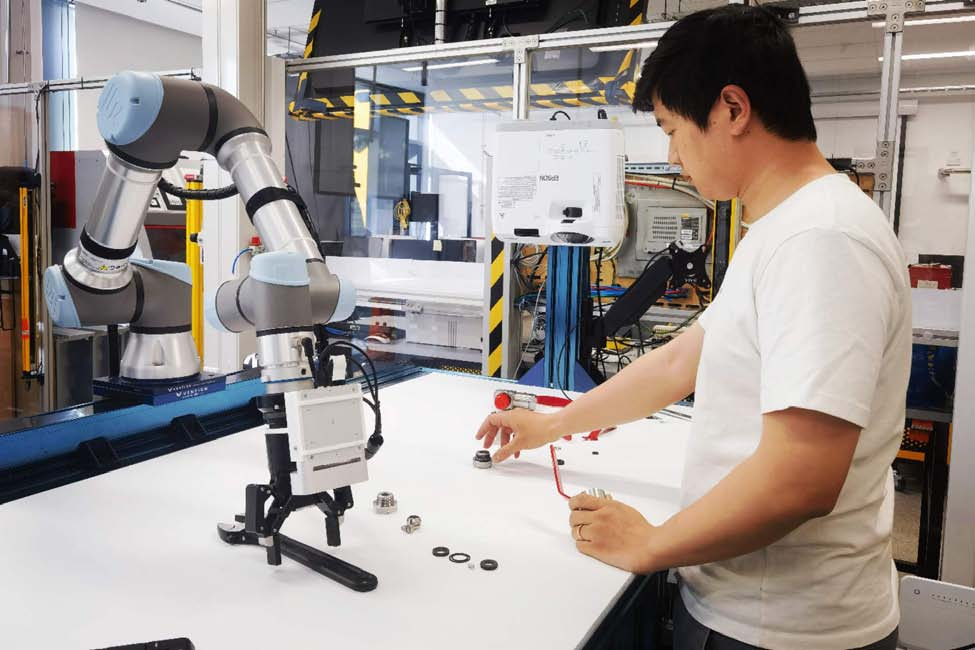
\includegraphics[width=0.72\textwidth]{figures/ur5e_platform_interim.png}
\end{kuetfigure}

The platform is a Universal Robots UR5e, a six-joint (6-DOF) collaborative arm
\cite{universalrobots2023ur5e}. It carries a payload of 5 kg to a reach of 850 mm, repeats a
taught position to within 0.03 mm, and weighs 20.6 kg unmounted. Every one of its six joints is
rated to the same maximum speed, 180 deg/s, which is exactly \(\pi\) rad/s. The simulated
arm in this thesis is capped at 3.14 rad/s for the same reason a real one is: past that speed the
motion stops being something a person nearby could react to in time. The provenance of that figure
matters: 3.14 rad/s is the datasheet limit itself, carried into the simulator so that a policy
trained there is never asked to move faster than the physical machine could follow it. The UR5e also ships with seventeen configurable safety
functions and is certified to the relevant collaborative-robot safety standards, ISO 13849-1
(Category 3, Performance Level d) and ISO 10218-1 \cite{universalrobots2023ur5e}. None of those
seventeen functions is exercised by the simulation. What this thesis borrows from the platform is
its physical envelope, its speed and reach limits, not its built-in safety controller, and
Chapter~\ref{ch:methods} is explicit about which of the two is under test.

Machines with this specification already do real work outside the laboratory. UR-class arms in
the UR5e's size class are common on production floors for exactly the tasks a 5 kg payload and an
850 mm reach suit: pick-and-place, machine tending, small-parts assembly and packaging, and
inspection stations where a part has to be picked up and held in front of a camera. The same
collaborative certification that lets one work next to a person on a line is also why it turns up
so often in research: it is affordable enough for a university laboratory, safety-rated enough to
run near people without a fenced cell, and common enough on real production floors that a result
obtained on one arm should say something useful about the rest of that population. Two of the
papers already cited in this chapter used a UR5-class arm for exactly that reason, one for
grasping \cite{ferreira2025grasping} and one for collision avoidance around a moving person
\cite{xia2024proactive}. The platform used here is drawn from that same working population.

Two further reasons fixed the choice. The preceding project in this laboratory used a
different, custom five-degree-of-freedom arm for classical visual servoing
\cite{khan2025csrt_ibvs}; this thesis moves to a UR-class platform because the safety question it
asks, how a learned policy behaves near a joint limit or a kinematic singularity, is best posed on
hardware whose limits and safety record are already public and well documented. Isaac Lab, the
simulation framework used throughout (Chapter~\ref{ch:methods}), also ships the UR5e as one of its
reference manipulators, so building the environment on this arm meant working from a supported
example rather than adapting a custom robot from scratch. The joint limits and speed ceiling used
throughout this thesis therefore belong to a machine that exists, not one assumed for convenience.

\section{Background}\label{sec:i-background}

Industrial manipulators increasingly work in spaces shared with people rather than behind a
fence, and the UR5e described above is a working example of that shift.
A controller that follows a fixed, hand-derived trajectory can be inspected and bounded before it
ever moves: an engineer can trace every configuration it will visit and check each one against a
joint limit or a known obstacle. A policy obtained by training a reinforcement learning agent
cannot be inspected the same way. Its behaviour is known only through the statistics of the
trajectories it produces during and after training, not through a proof that covers every
configuration it might reach. Safe operation of a UR-class collaborative arm around people is
already treated as a live industrial requirement, not a hypothetical one \cite{xia2024proactive}.
Reinforcement learning is attractive for manipulation precisely because it can learn grasping and
placement behaviour directly from experience, without a hand-built controller for every object and
pose the arm might encounter. What that learned behaviour does in the configurations it visits
rarely, however, is not a detail to be checked after the fact. For a policy sharing a workspace
with a person, it is the condition deployment depends on.

The standard formulation of reinforcement learning gives a designer only one channel for stating
what the agent should avoid: the reward function. Take the UR5e's own joint-speed ceiling as a
concrete case. A designer who wants the trained policy to respect it has, in the standard
formulation, exactly one lever: add a penalty term for exceeding it, sized by a weight that trades
a unit of excess speed against a unit of task reward. That weight has to be fixed before training
starts, before the designer has any real sense of how large a violation the untrained policy will
produce or how much task performance the penalty will cost once it starts to bind. Set the weight
too small and the constraint is decorative. Set it too large and the agent may refuse to move at
all. An alternative, pursued in this thesis, is to keep the requirement outside the reward
entirely and state it instead as a constraint with an explicit budget: a quantity that can be set
from a measurement of the system, such as the arm's own rated limits, and checked afterwards
against what the trained policy actually used \cite{achiam2017cpo}. The distinction matters
because of what each side has to answer for. A reward weight is a guess, tuned by trial and error
against whatever the agent happens to do. A constraint budget is a number the designer can defend
before training ever starts, because it comes from a measurement rather than a hunch.
Chapter~\ref{ch:litreview} reviews this distinction, and the literature built on either side of
it, in full.

\section{Problem Description}\label{sec:i-problem}

This thesis puts that alternative to a direct test. It trains a UR5e in simulation to pick up and
lift a cube, comparing a standard proximal policy optimisation (PPO) agent against a constrained
variant of the same algorithm (PPO-Lagrangian) under a shared floor on manipulability, a measure of
how far a configuration sits from a kinematic singularity. Such a comparison, as usually run in the
literature, has two problems.

\begin{itemize}
  \item \textbf{The cost-critic confound.} Adding a constraint to an RL agent does not add only a
  constraint. A Lagrangian method also adds a cost critic, a second value network trained
  alongside the policy to estimate the constraint violation the current policy would incur. That
  network is present whether or not the constraint is actively binding, and its presence can
  influence training through machinery the two agents no longer share. A comparison that trains
  only the unconstrained baseline and the fully constrained agent cannot separate what the
  constraint achieved from what the extra network alone changed.
  \item \textbf{Seed variance.} A single training run under one random seed says little about what
  a method will do on the next run \cite{henderson2018matters}. Published comparisons of
  constrained against unconstrained manipulation policies typically report one run, or a mean over
  few, without a measure of how much the outcome would vary if the same method were retrained.
\end{itemize}

Section~\ref{sec:b-gap} sets out this gap in full against the closest published comparison
\cite{khan2026rl_precision_grasping}. What matters here is the consequence for design.
Chapter~\ref{ch:methods} describes a comparison built to answer both problems at once. Alongside
the unconstrained baseline it places a control arm, identical to the constrained agent in every
respect except that its Lagrange multiplier is pinned to zero, so that whatever the cost critic
does on its own can be measured apart from whatever the constraint does. The constrained agent is
trained at two episodic cost budgets, 25 and 15, because a tighter budget and a looser one make
different demands of the policy. Every arm is trained on five independent random seeds, and every
reported quantity carries its spread across those seeds instead of standing as a single number.

The control arm turned out to reproduce the unconstrained baseline exactly, at the level of the
stored network weights rather than merely to within statistical noise, so the two are reported
jointly as a single arm throughout Chapter~\ref{ch:results}. The isolation this design was built
to provide therefore measures the cost critic's independent effect as exactly zero, and
Section~\ref{sec:r-validity} gives that verification in full. Three arms are reported in the end:
the joint baseline, and the constrained agent at each of its two budgets.

The work also continues a line of manipulator research from the same laboratory. The preceding
study \cite{khan2025csrt_ibvs} addressed the perception and motion side of manipulation, tracking
and following a target with classical image-based visual servoing. This thesis addresses the
control policy instead, with reinforcement learning, and adds a safety constraint that a classical
visual servoing loop does not itself provide.

\section{Objectives}\label{sec:i-objectives}

The general objective of this thesis is to determine whether expressing a manipulability safety
requirement as an explicit constraint, rather than as a term in the reward, changes the safety
behaviour of a learned grasping policy on a UR5e manipulator, and whether it changes how
predictable that behaviour is across independent training runs.

The specific objectives are as follows:

\begin{itemize}
  \item To implement an unconstrained PPO baseline and a constrained PPO-Lagrangian agent for a
  UR5e pick-and-lift grasping task in Isaac Lab, trained under a shared floor on manipulability.
  \item To isolate the effect of the constraint from the effect of the cost critic that implements
  it, by training a control arm that carries the cost critic with its Lagrange multiplier held at
  zero throughout training.
  \item To establish whether the constrained agent's behaviour depends on how tight its budget is,
  by training it at two episodic cost budgets, 25 and 15, instead of one.
  \item To train every arm on five independent random seeds and report task performance and safety
  outcomes as a distribution across those seeds instead of as a single mean.
  \item To evaluate every trained policy on frozen, held-out episodes, so that the reported safety
  and task figures describe the policy that would actually be deployed rather than a
  still-learning one.
  \item To determine, from the resulting distributions, whether the constraint changes the average
  safety outcome of a training run, the spread of that outcome across runs, or both.
\end{itemize}

\section{Scope}\label{sec:i-scope}

This thesis was registered under the title \textit{Safe Adaptive Image-Based Visual Servoing with
Constrained Reinforcement Learning for Precision Grasping on a UR5 Manipulator: From Simulation to
Real Hardware}, and was proposed as a three-layer programme, not as Layer 1 alone. The title on
this book is narrower because the delivered work is narrower, and the paragraphs below say exactly
where the boundary falls.

Layer 1, delivered here, is safe reinforcement learning for grasping in simulation, using
privileged pose information rather than vision. Layer 2 would have closed the loop with vision: an
image-based visual servoing scheme in which the image Jacobian relating pixel motion to joint
motion is tuned by the learned policy rather than fixed in advance, replacing the privileged pose
feedback of Layer 1 with an eye-in-hand RGB-D camera and object detection. It would have been a
direct upgrade of the predecessor project in this laboratory, which used a fixed, hand-derived
image Jacobian for the same visual-servoing task \cite{khan2025csrt_ibvs}. Layer 3 would have
carried the resulting controller onto the physical UR5e over ROS 2, closing the gap between the
Robotiq 2F-85 gripper modelled in simulation and the different gripper fitted to the laboratory's
real arm.

Only Layer 1 is delivered. Layers 2 and 3 are not attempted, and that is stated here as a
deliberate narrowing of scope, decided against a fixed submission date, rather than as an unmet
target. Building an evaluation protocol able to separate a safety constraint's effect from an
implementation artefact, and to characterise it across independent seeds, could not be done to a
defensible standard alongside two further systems-integration efforts of comparable size. Both
dropped layers are carried forward as future work in Chapter~\ref{ch:conclusion}.

Layer 1 on its own remains a substantial question. Constraining a policy's behaviour with an explicit
safety budget, rather than through a shaped reward, is already active practice on UR-class
hardware doing collision avoidance around a moving person \cite{xia2024proactive}, and on other
manipulator platforms doing constrained grasping specifically \cite{khan2026rl_precision_grasping}.
What this thesis contributes sits inside that same practice: a comparison protocol for measuring
what the constraint itself does, isolated from an implementation artefact and reported across
seeds rather than as a single run, on a platform common enough in both industry and the published
literature that the result should say something beyond this one laboratory's copy of it.

Within Layer 1, the scope is:

\begin{itemize}
  \item \textbf{Task.} Single-object pick-and-lift grasping on a simulated UR5e in Isaac Lab, on
  the weld-grasp environment described in Chapter~\ref{ch:methods}. The gripper is present and
  driven, but the moment of contact is abstracted rather than modelled as a full physical grasp.
  \item \textbf{Comparison.} Three algorithm arms: an unconstrained PPO baseline and two
  PPO-Lagrangian variants at different cost budgets, each trained on five independent random
  seeds.
  \item \textbf{Safety quantity.} A single constrained quantity, a floor on manipulability.
  Joint-limit proximity and workspace clearance are measured and reported but are not themselves
  constrained.
  \item \textbf{Evaluation.} The frozen policy produced by each run, assessed on held-out episodes
  with the multiplier and exploration noise fixed, not the training-time behaviour of a policy
  still being updated.
  \item \textbf{Algorithms.} The comparison uses established methods, PPO and PPO-Lagrangian; it
  does not propose a new constrained-RL algorithm. The contribution claimed is the comparison
  protocol and what it finds, not a new optimiser.
  \item \textbf{Hardware validation.} All results are produced in simulation. No policy from this
  thesis is run on the physical UR5e. That step belongs to Layer 3, out of scope here and named as
  future work in Chapter~\ref{ch:conclusion} rather than as a claim already tested.
\end{itemize}

% \chapter{Literature Review}\label{ch:litreview}

\begin{draftnote}
MODULE 3 --- first draft, written 2026-08-02 (Day 25, evening).

\textbf{The old ``BLOCKED: no reference PDFs are in this repo'' note is superseded and has been
deleted.} The chapter is written from the 21 verified entries in \texttt{references.bib} against
the spine agreed in \texttt{logbook/10\_references.md}. Every citation here appears in that claim
map; if a new claim is added, add its row to the map first.

\textbf{Claim discipline used.} Load-bearing technical claims are drawn from the constrained-RL
foundations and from the three papers held in full (\cite{khan2026rl_precision_grasping},
\cite{shahid2022continuous_grasping}, \cite{ferreira2025grasping}). The surveys and application
papers are cited for framing, taxonomy and positioning only, and no specific numerical result is
attributed to a paper not held. Section~\ref{sec:b-gap} is load-bearing --- it is where the gap
statement is made, and Chapter~\ref{ch:intro} should restate it.

\textbf{Open for revision:} target is 8--10 pages, check against the built PDF. Consider whether
Section~\ref{sec:b-repro} belongs here or in Chapter~\ref{ch:methods} --- it is placed here
because it motivates the ten-seed protocol, but it is arguably method rather than background.
\end{draftnote}

\section{The safety requirement in learned manipulation}\label{sec:b-motivation}

A robot manipulator that learns its own control policy poses a problem that a manipulator running
a hand-written controller does not. The behaviour of a classical controller can be inspected,
bounded and argued about before the machine is switched on; the behaviour of a policy obtained by
reinforcement learning is a consequence of an optimisation run, and is known only through the
statistics of the trajectories it produces. When such a policy is to be deployed on a physical arm
sharing its workspace with people, equipment or the workpiece itself, the question of what it does
in the configurations it visits rarely is not a secondary concern. It is the condition on which
deployment depends at all.

The difficulty is that reinforcement learning, in its standard form, offers a single channel
through which a designer expresses what the agent should and should not do: the reward function.
Safety requirements expressed through that channel become penalty terms, and a penalty term must
be given a weight. That weight is a trade-off rate between task performance and safety which the
designer must fix before knowing what either will be worth, and which has no natural units --- it
is a number tuned until the resulting behaviour looks acceptable. Achiam \emph{et al.}
\cite{achiam2017cpo} make this argument directly in motivating constrained policy optimisation:
for systems that interact physically with or around humans, it is more natural to specify a reward
function \emph{and} a set of constraints than to encode both into one scalar objective.

The alternative is to keep the safety requirement outside the reward and impose it as a constraint
with a budget. A budget has a property the weight does not: it can be stated in advance, in the
units of the quantity being constrained, and it can be audited afterwards against what the trained
policy actually spent. This distinction --- \emph{a shaped reward requires the designer to guess a
weight, a constraint requires only that they state a limit} --- is the premise of this thesis, and
Section~\ref{sec:b-manip} shows that it separates two otherwise similar bodies of work on
singularity avoidance.

This chapter reviews the literature establishing that premise and locates this thesis within it.
Section~\ref{sec:b-saferl} introduces safe reinforcement learning and the taxonomy under which
this work falls. Section~\ref{sec:b-cmdp} gives the constrained Markov decision process, the
formalism used throughout. Section~\ref{sec:b-cpo} covers the deep constrained policy optimisation
algorithms from which the constrained agent is taken. Section~\ref{sec:b-roboticsafety} turns to
safety in robot learning specifically, and Section~\ref{sec:b-manipulation} to reinforcement
learning on manipulators and on the UR5 in particular. Section~\ref{sec:b-manip} treats
manipulability and singularity avoidance, the operative safety quantity of this work.
Section~\ref{sec:b-repro} addresses seed variance. Section~\ref{sec:b-gap} states the gap this
thesis addresses.

\section{Safe reinforcement learning}\label{sec:b-saferl}

Safe reinforcement learning is the study of methods that optimise a policy while respecting some
notion of acceptable behaviour during learning, at deployment, or both. The organising survey of
the field is that of García and Fernández \cite{garcia2015survey}, which divides the literature
into two branches according to where the safety requirement is inserted. The first modifies the
\emph{optimisation criterion}, so that the objective the agent maximises is itself changed --- by
a risk-sensitive transformation, by a worst-case criterion, or by the addition of explicit
constraints. The second modifies the \emph{exploration process}, leaving the objective intact but
restricting or guiding the actions the agent may try, typically using external knowledge such as a
teacher, a demonstration set or a backup controller.

This thesis belongs to the first branch, and to its constrained-criterion sub-family in
particular. The distinction matters for reading Chapter~\ref{ch:results}: methods in the second
branch aim to make the learning process itself safe and are evaluated on violations accumulated
\emph{during} training, whereas methods in the first aim to produce a policy that satisfies a
requirement once trained, and are properly evaluated on the frozen policy. The evaluation protocol
of this work follows the latter convention, and Section~\ref{sec:r-design} explains why an earlier
version of these results, which read safety figures from training-time telemetry, was withdrawn.

The more recent review by Gu \emph{et al.} \cite{gu2024review} surveys the field after the
deep-learning era and reports that the constrained-criterion approach, expressed as a constrained
Markov decision process, has become the prevailing formalism for safe reinforcement learning. That
observation places the present work inside the mainstream of the field rather than at its margin,
and it is why the CMDP is adopted here without further argument.

\begin{kuettable}{Where the safety requirement is inserted: the two branches of safe
reinforcement learning.}{tab:b-taxonomy}
\begin{tabular}{p{3.1cm}p{4.7cm}p{4.4cm}}
\hline
\textbf{Branch} & \textbf{Mechanism} & \textbf{Evaluated on} \\
\hline
Modify the optimisation criterion & Risk-sensitive or worst-case objectives; explicit constraints
on expected cumulative cost & The trained policy, on held-out episodes \\
Modify the exploration process & Teacher guidance, demonstrations, backup controllers, action
shielding & Violations accumulated during training \\
\hline
\end{tabular}
\end{kuettable}

\section{The constrained Markov decision process}\label{sec:b-cmdp}

The formal object underlying the constrained-criterion branch is the constrained Markov decision
process, developed in its modern form by Altman \cite{altman1999cmdp}. A standard Markov decision
process is the tuple (S, A, P, r, \(\gamma\)) over a state space S, an action space A, a transition
kernel P, a reward function r and a discount factor \(\gamma\). A CMDP augments this with a cost
function c and a budget d, and asks for a policy maximising expected return subject to a bound on
expected cumulative cost. Chapter~\ref{ch:methods} states the optimisation problem in full; what
matters here is what the formalism buys.

Two properties are relevant. The first is that the safety requirement is expressed in the units of
the cost rather than in units of reward, so it can be set from a measurement of the system rather
than from a tuning exercise --- the calibration procedure of Section~\ref{sec:m-calib} depends on
this. The second is that the constrained problem admits a Lagrangian relaxation, in which the
constraint is folded into the objective through a multiplier \(\lambda\) that is itself optimised.
The duality theory licensing that treatment is the contribution of \cite{altman1999cmdp}, and it is
what makes the algorithms of the next section possible: rather than solving a constrained problem
directly, they solve a sequence of unconstrained problems in which the penalty weight is not
guessed by the designer but driven by the observed violation.

That last point deserves emphasis, because it is easily lost. A Lagrangian method does end up
optimising a weighted sum of reward and cost, which superficially resembles reward shaping. The
difference is that the weight is not a hyperparameter. It is a dual variable that rises while the
budget is exceeded and falls once it is met, so the designer specifies the budget and the optimiser
discovers whatever weight is required to satisfy it.

\section{Constrained policy optimisation in deep reinforcement learning}\label{sec:b-cpo}

The policy-gradient algorithm used as the baseline throughout this thesis is proximal policy
optimisation \cite{schulman2017ppo}, which limits the size of each policy update through a clipped
surrogate objective and has become the default on-policy method for continuous control. Its
popularity is partly a matter of robustness: it attains much of the reliability of trust-region
methods at a fraction of their implementation complexity, which is also why it is the algorithm
most commonly extended when a constraint is to be added.

Constrained policy optimisation (CPO) \cite{achiam2017cpo} was the first algorithm to bring the
CMDP into deep reinforcement learning at scale. It extends the trust-region approach so that each
update both improves the return and maintains approximate constraint satisfaction, computing a
penalty coefficient afresh at every step. Its significance for this thesis is as much conceptual as
algorithmic: it established the constrained formulation as a practical alternative to reward
shaping for high-dimensional continuous control, and it supplies the motivating argument quoted in
Section~\ref{sec:b-motivation}.

The algorithm actually implemented here, however, is the Lagrangian variant of PPO, as specified in
the Safety Gym benchmark report of Ray \emph{et al.} \cite{ray2019benchmarking}. That report
proposes constrained reinforcement learning as the standard formalism for safe exploration and
supplies a benchmark suite of continuous-control environments together with reference
implementations of PPO, TRPO, their Lagrangian forms, and CPO. Two of its findings bear directly on
the design of this study. The first is the specification itself: the constrained agent studied here
is PPO-Lagrangian as defined in \cite{ray2019benchmarking}, in which an adaptive penalty on the
safety cost is maintained by dual ascent on a Lagrange multiplier. The second is empirical, and is
the reason PPO-Lagrangian was preferred to CPO --- \cite{ray2019benchmarking} reports that CPO
performs poorly on the Safety Gym environments by comparison with the considerably simpler
Lagrangian methods. Given that result, adopting CPO would have required a justification this work
does not have; the Lagrangian form is both easier to implement correctly and better supported by
the published comparison.

Lagrangian methods carry a characteristic weakness, and this thesis encounters it directly in
Chapter~\ref{ch:results}. Because the multiplier is updated by plain dual ascent, its trajectory
oscillates: it rises while the cost exceeds the budget, overshoots, and decays once the cost has
been driven under. Stooke \emph{et al.} \cite{stooke2020pid} analyse this behaviour and propose
treating the multiplier update as a control problem, adding proportional and derivative terms to
damp the oscillation. Their analysis is used in Section~\ref{sec:r-variance} to interpret the
multiplier values observed at the end of training, and the PID form itself is identified in
Chapter~\ref{ch:conclusion} as the natural extension of this work.

The benchmarking landscape has since consolidated. Safety Gymnasium \cite{ji2023safetygymnasium}
supersedes the original Safety Gym environments and ships alongside a library of safe reinforcement
learning algorithms under a common evaluation protocol. Its reporting conventions --- episodic cost
against a stated budget, and violation rates measured per episode --- are those adopted in
Chapter~\ref{ch:results}.

\section{Safety in robot learning}\label{sec:b-roboticsafety}

The literature reviewed so far approaches safety from the machine-learning side. Robotics
approaches it from the control side, with a vocabulary of invariant sets, barrier certificates and
stability guarantees that developed independently. Brunke \emph{et al.} \cite{brunke2022safe}
survey the intersection and, more usefully for the present purpose, reconcile the two vocabularies
into a common framework spanning learning-based control through to safe reinforcement learning.

That reconciliation is necessary here because this thesis sits across the boundary. The quantities
constrained in this work --- the manipulability measure, the distance to a joint limit, the
clearance above the work surface --- are control-theoretic constructs describing the kinematic
state of the arm. The mechanism enforcing them is a learning-theoretic one: a cost critic and a
dual variable. Neither literature alone supplies the language for that combination.

The survey also draws a distinction that constrains what may be claimed from the results of this
work. Methods enforcing a constraint in expectation, as a Lagrangian method does, bound
\emph{expected} exposure to unsafe configurations; they do not bound the severity of any individual
excursion. Methods supplying a safety certificate, such as a control barrier function acting as a
filter on the commanded action, offer the latter guarantee but require a model. This distinction is
returned to in Section~\ref{sec:r-safety}, where a counter-result of exactly this shape is
reported, and in Chapter~\ref{ch:conclusion}, where the two mechanisms are argued to address
different halves of the problem.

Within manufacturing specifically, Elguea-Aguinaco \emph{et al.} \cite{elguea2023review} review
reinforcement learning for contact-rich manipulation from 2017 onward, covering reward design,
sim-to-real transfer and the treatment of safety. Their survey is used in Chapter~\ref{ch:methods}
to establish which of the design choices made in this work follow established practice.

\section{Deep reinforcement learning for robotic manipulation}\label{sec:b-manipulation}

Applications of deep reinforcement learning to manipulation divide broadly by algorithm family.
Shahid \emph{et al.} \cite{shahid2022continuous_grasping} compare an on-policy method (PPO) against
an off-policy method (soft actor-critic) on a grasping task with a Franka Emika Panda, using a
dense reward and a fine-tuning procedure that adapts a trained policy to a modified task. The study
is relevant here in three ways: it is the methodological template for an on-policy versus
off-policy comparison on a manipulation task; it demonstrates transfer of the learned behaviour
from simulation to a physical robot, which supports the position taken in
Chapter~\ref{ch:conclusion} that results of this kind are transferable in principle; and it is the
precedent for the off-policy arm that was planned for this study and ultimately not trained, as
recorded in Section~\ref{sec:r-limits}.

Work specific to the UR5 platform is less common. Ferreira and Barbosa \cite{ferreira2025grasping}
train a UR5 fitted with a Robotiq 2F-85 gripper to grasp randomly positioned objects in a PyBullet
environment, comparing soft actor-critic against PPO under a reward combining distance penalties
with grasp and pose terms. They report grasp success rates of 87\,\% for SAC and 82\,\% for PPO.
These are the closest published figures for a learned UR5 grasping policy, and they are quoted here
with one qualification that must be carried into any comparison: their task requires a full
physical grasp, in which the fingers close on the object and the resulting contact must be stable,
whereas the task studied in this thesis abstracts the grasp as a weld for the reasons given in
Section~\ref{sec:m-env}. The success rates of Chapter~\ref{ch:results} are therefore not directly
comparable to theirs, and are not presented as though they were.

On the safety side, Xia \emph{et al.} \cite{xia2024proactive} apply deep reinforcement learning to
proactive obstacle avoidance for a UR5e in a human-robot collaborative assembly setting, with depth
sensing for environmental perception and a wrist force-torque sensor. Their work establishes that
safe operation of this specific manipulator is an active industrial concern rather than an academic
construction, which is the premise on which the practical relevance of this thesis rests.

\section{Manipulability and singularity avoidance}\label{sec:b-manip}

The operative safety constraint in this thesis is a floor on manipulability. The measure is due to
Yoshikawa \cite{yoshikawa1985manipulability}, who proposed \(w = \sqrt{\det(JJ^{\top})}\), computed
from the manipulator Jacobian J, as a scalar index of a configuration's capacity to generate
end-effector motion in arbitrary directions. The index falls towards zero as the arm approaches a
kinematic singularity, at which it loses the ability to move instantaneously along some Cartesian
direction and at which small commanded end-effector velocities map to large joint velocities. It is
the standard measure of this property and is used throughout this work; Chapter~\ref{ch:methods}
defines the cost term built from it.

Singularity avoidance has been treated within learning frameworks before, and the manner of that
treatment is precisely where this thesis differs. Shen \emph{et al.} \cite{shen2022reactive}
address reactive obstacle avoidance for redundant manipulators by learning motion in the null space
of the Jacobian, and introduce the manipulability index \emph{into the reward function} so that the
arm maintains a well-conditioned posture while executing its task. The approach is sound and the
objective is the same as the one pursued here. The mechanism is not. Placing manipulability in the
reward requires a weight relating a unit of manipulability to a unit of task progress, and that
weight is a design choice with no principled setting. Placing it in a constraint, as this thesis
does, requires instead a budget --- a statement of how much cumulative proximity to singularity an
episode may incur --- which can be measured from a baseline policy and audited against the trained
one.

The comparison is worth stating plainly, because it is the sharpest available expression of what
this thesis does differently. Both approaches seek the same behaviour. One obtains it by tuning a
trade-off; the other by declaring a limit.

\section{Reproducibility and seed variance}\label{sec:b-repro}

A final strand of the literature is methodological rather than algorithmic, and it bears on the
central experimental finding of this work. Henderson \emph{et al.} \cite{henderson2018matters}
examine the reproducibility of results in deep reinforcement learning and demonstrate that outcomes
for a single algorithm on a single task can differ substantially according to the random seed
alone, independently of any change to the algorithm, its hyperparameters or the environment. Their
recommendation is that results be reported over multiple independent seeds with a measure of
dispersion, and that comparisons between methods be treated with corresponding caution.

Two consequences follow for this thesis. The first is procedural: the protocol of
Chapter~\ref{ch:methods} trains every arm on ten independent seeds and reports dispersion across
them rather than a single figure, and that protocol is justified by reference to
\cite{henderson2018matters} rather than by assertion. The second is interpretive: the seed-to-seed
spread reported in Section~\ref{sec:r-variance} is not an anomaly of this environment but an
instance of a documented property of the method, which is why it is presented there as a measured
quantity rather than as a surprising discovery.

\section{Research gap and positioning}\label{sec:b-gap}

The nearest published analogue to the present study is that of Khan \emph{et al.}
\cite{khan2026rl_precision_grasping}, which compares a model-free PPO baseline against its
constrained variant for precision grasping and safety-critical coordination on a robotic arm, using
the Safety Gym framework extended with a Panda manipulator, and introduces a tactile feedback
scheme to accelerate learning under safety compliance. It is the closest match in method, in
framing and in intent, and this thesis should be read as continuing that line of work rather than
as departing from it.

Two gaps are nonetheless visible in that line, and it is these the present study addresses.

The first is a matter of experimental control. A constrained agent of this family differs from its
unconstrained baseline in more than the constraint: it constructs and trains an additional cost
critic, whose presence can perturb the optimiser through shared machinery even when the constraint
itself is inactive. Unless a third arm is trained that carries the cost critic but pins the
multiplier to zero, any measured difference between the constrained agent and the baseline sums two
effects of different kinds, and cannot be attributed to the constraint alone. Published comparisons
in this area, including \cite{khan2026rl_precision_grasping}, do not report such a control arm.
Chapter~\ref{ch:results} shows this is not a hypothetical concern: an earlier version of the
present work reported a large advantage for the constrained agent that was subsequently traced to
exactly this class of implementation artifact and withdrawn in full.

The second is a matter of dispersion. Comparisons in this literature are typically reported as
means, without an account of how much the outcome varies across training runs differing only in
their random seed. Given the finding of \cite{henderson2018matters} discussed in
Section~\ref{sec:b-repro}, a mean taken over few seeds is a weak basis for a safety claim: an
integrator deploying such a policy does not obtain the mean over training runs they will never
perform, but the single policy they happened to train. Whether a safety constraint changes the
\emph{predictability} of the outcome, and not merely its average, is therefore a question of
practical consequence, and it is not one the existing literature answers.

This thesis addresses both. It trains a three-arm comparison --- an unconstrained baseline, a
control arm carrying the cost critic with the multiplier pinned to zero, and the constrained agent
--- on ten independent seeds each, and reports the decomposition of the constrained-versus-baseline
difference into an implementation term and a constraint term, together with the dispersion of every
reported quantity across seeds.

The work is also positioned locally. It continues a line of manipulator research in the same
laboratory, of which the immediately preceding study \cite{khan2025csrt_ibvs} implemented classical
image-based visual servoing with CSRT tracking on a five-degree-of-freedom manipulator. Where that
work addressed the perception and servoing loop with classical methods, the present work addresses
the control policy with learned ones, and adds the safety constraint that classical visual servoing
does not itself provide.

\section{Summary}\label{sec:b-summary}

Safety requirements on a learned manipulation policy are poorly served by reward shaping, which
obliges the designer to fix a trade-off weight in advance, and are better expressed as constraints
with stated budgets \cite{achiam2017cpo}. The constrained Markov decision process
\cite{altman1999cmdp} is the formalism for this, and is the prevailing one in contemporary safe
reinforcement learning \cite{gu2024review}. Among the deep algorithms implementing it, the
Lagrangian variant of PPO \cite{schulman2017ppo, ray2019benchmarking} is both simpler than the
trust-region alternative \cite{achiam2017cpo} and better supported by the published benchmark
comparison, and is the algorithm adopted here.

Applied to manipulators, this machinery has been used for obstacle avoidance and for grasping, on
the UR5 among other platforms \cite{ferreira2025grasping, xia2024proactive}, and singularity
avoidance in particular has been pursued by placing the manipulability measure
\cite{yoshikawa1985manipulability} inside the reward \cite{shen2022reactive}. This thesis places it
inside a constraint instead. Two gaps in the nearest published comparison
\cite{khan2026rl_precision_grasping} define the contribution: the absence of a control arm
isolating the effect of the cost critic from the effect of the constraint, and the absence of any
account of seed-to-seed dispersion. Chapter~\ref{ch:methods} sets out the method by which both are
addressed.


% Keep Methodology at 3 and Results at 4 while 1-2 are missing, so the
% numbering in the draft matches the numbering in the prose.
% DELETE this line the moment chapters/01 and chapters/02 are uncommented.
\setcounter{chapter}{2}

\chapter{Research Methodology}\label{ch:methods}

\begin{draftnote}
MODULE 4 --- needs restructuring, not just revising.

Ported from \texttt{Thesis\_Documentation/Methods\_Chapter\_Layer1.md} (draft 2026-07-19), which
is now a frozen dated record; this \texttt{.tex} is the source of truth. Numbers verified against
\texttt{ur5\_grasp/} source on 2026-07-19.

\textbf{This chapter is currently too big for its slot.} Under the KUET seven-chapter structure
it should hold only the method: the CMDP formulation, the design of the safety cost, and the
constrained optimisation algorithm. The environment, robot model, observation/action/reward,
threshold calibration and the training and evaluation protocol all belong in
Chapter~\ref{ch:setup}, and the software realisation belongs in Chapter~\ref{ch:implementation}.
Split before writing anything new.

\textbf{Also open:} this draft predates the Day-23 audit. Check whether it narrates the
withdrawal, since Section~\ref{sec:r-validity} of the results chapter assumes it does.
\end{draftnote}

\section{Problem formulation}\label{sec:m-cmdp}

The grasping task is posed as a constrained Markov decision process (CMDP). A standard MDP is the
tuple (S, A, P, r, \(\gamma\)) over states S, actions A, transition kernel P, reward r and discount \(\gamma\); a CMDP
augments it with a cost function c and a budget d, and asks the policy to maximise expected return
while keeping expected cumulative cost bounded:

\begin{equation}
  \max_{\pi}\ \mathbb{E}\!\left[\sum_{t}\gamma^{t} r(s_t,a_t)\right]
  \quad\text{subject to}\quad
  \mathbb{E}\!\left[\sum_{t} c(s_t,a_t)\right] \le d .
  \label{eq:cmdp}
\end{equation}

This framing separates \emph{what the robot should achieve} (grasp and place the cube, encoded in r) from
\emph{what it must not do} (enter unsafe configurations, encoded in c). The remainder of this chapter
defines the simulation environment and MDP (Section~\ref{sec:m-env}), the safety cost that instantiates c
(Section~\ref{sec:m-cost}), the constrained optimisation algorithm that solves the CMDP (Section~\ref{sec:m-cppo}), the calibration
that makes the constraint meaningful (Section~\ref{sec:m-calib}), and the training and evaluation protocol
(Sections~\ref{sec:m-train}--\ref{sec:m-eval}).

\section{Simulation environment and task}\label{sec:m-env}

Experiments are carried out in NVIDIA Isaac Sim 5.0.0 with the Isaac Lab 2.3.0 manager-based
framework, using the \texttt{rsl\_rl} 3.0.1 reinforcement-learning library, PyTorch 2.7 (CUDA 12.8) and a
single RTX 5090 GPU. The task is retargeted from Isaac Lab's Franka cube-lift environment onto a
Universal Robots UR5e equipped with a Robotiq 2F-85 gripper; only the robot, action space, and
end-effector frame are changed, so the reward shaping and task structure of the well-tested base
environment are preserved.

The manipulator is a six-degree-of-freedom arm controlled by joint-position commands on its six
revolute joints (shoulder pan, shoulder lift, elbow, and three wrist joints), with the action scaled
by 0.5 about the default configuration. The gripper is driven by a single binary open/close command
on the Robotiq actuation joint. The object is a rigid cube (Isaac's DexCube asset scaled to 0.8)
initialised on a table in front of the arm, and its target is a goal pose sampled once per episode.

Because the Robotiq 2F-85 is a closed-loop linkage whose passive finger joints transmit no normal
force to the pads in simulation, contact-based grasping does not hold the cube (verified with
\texttt{grasp\_hold\_test.py}: the cube falls through the fingers regardless of clamp force). A subsequent
diagnostic (\texttt{tools/check\_gripper\_mount.py}) identified the underlying mechanism: in the converted
USD asset, all nine gripper rigid bodies are reported by the physics articulation view at positions
coincident with the \texttt{wrist\_3\_link} origin, rather than distributed along the 150 mm gripper body.
The pad-to-pad separation is nevertheless reproduced correctly (84.4 mm measured against an 85 mm
specification stroke), confirming that the gripper's internal linkage is intact while its transform
relative to the wrist is degenerate. Finger contact therefore cannot resolve at the location where
the gripper geometry is rendered, which fully accounts for the observed pass-through behaviour.

Since the Layer 1 safe-RL result is independent of the specific grasp mechanism, the gripper is
modelled as a lumped mass at the wrist flange and contact grasping is replaced by a \emph{proximity-weld}
abstraction. The tool centre point is defined kinematically as a fixed 160 mm offset along the
\texttt{wrist\_3\_link} approach axis --- the position a correctly mounted 2F-85 pad midpoint would occupy ---
and when the policy commands a close action while the cube lies within a 6 cm tolerance of that
frame, the cube latches and its pose tracks the end-effector each control step (with its velocity
zeroed); an open command releases it and physics resumes. This makes ``grasp-and-lift'' reliable so
that both the baseline and the constrained policy can learn the task, and defers realistic finger
contact to the Layer 3 sim-to-real work.

Two consequences of this abstraction are stated explicitly. First, the lumped-mass gripper alters
the wrist inertia relative to a fully articulated model; because the same asset is used for every
run in the benchmark, this affects all algorithms identically and does not confound the comparison.
Second, self-collision is disabled in simulation and the collision cost term is a table-plane
keep-out rather than a link-pair check, so learned configurations are not guaranteed to be
self-collision-free on hardware. Both are revisited in the Limitations discussion.

\subsection{State, action, and reward}\label{sec:m-mdp}

The policy receives a privileged observation comprising the arm joint positions and velocities
(relative to their defaults), the cube position expressed in the robot base frame, the commanded goal
position, and the previous action. Object pose is provided directly rather than through vision, which
isolates the safe-RL contribution from perception; closing the loop with an image-based estimate is
the subject of Layer 2. All observation terms are clamped to a finite range as a numerical
safeguard, preventing a single transiently-unstable environment from corrupting the on-policy batch.

The action is the six-dimensional vector of target arm-joint positions together with the binary
gripper command. Episodes last five simulated seconds with a control decimation of two physics steps
per action, and the goal pose is resampled once per episode from a uniform range over the workspace
(x \(\in\) {[}0.4, 0.6{]} m, y \(\in\) {[}\(-\)0.25, 0.25{]} m, z \(\in\) {[}0.25, 0.5{]} m). At reset the cube position is randomised
within a small planar region so the policy cannot memorise a fixed trajectory.

The reward is the shaped sum inherited from the base lift task: a reaching term that rewards reducing
the end-effector-to-object distance (tanh kernel, standard deviation 0.1, weight 1), a lifting term
that rewards raising the cube above 0.04 m (weight 15), and two goal-tracking terms that reward
bringing the lifted cube toward the commanded goal at coarse and fine scales (tanh kernels with
standard deviations 0.3 and 0.05, weights 16 and 5). Small quadratic penalties on the action rate and
joint velocity (each weight \(-\)\(10^{-4}\)) discourage jerky motion. Crucially, the reward contains \textbf{no
safety term} --- safety is expressed entirely through the separate cost channel of Section~\ref{sec:m-cost}, so that
the comparison in the Results chapter isolates the effect of the constraint.

\section{The safety cost function}\label{sec:m-cost}

Safety is encoded by a per-step cost computed in \texttt{SafetyCostComputer} (\texttt{safe\_rl/costs.py}) from three
geometric-kinematic terms. Each term is zero while the arm is safe and grows smoothly as the arm
enters a danger zone; smoothness matters because it gives the cost critic (Section~\ref{sec:m-cppo}) a usable
gradient. The three terms are summed into a single aggregate cost so that a single Lagrange multiplier
governs the whole constraint, and each term additionally exposes a mean value and a binary violation
indicator for reporting.

The first term is a \textbf{collision keep-out}. For each monitored arm link (forearm, wrist-1, wrist-3)
the penetration depth below the table plane, max(z\_floor \(-\) z, 0), is summed across links, with the
table plane at z\_floor = 0. Because self-collisions are disabled in simulation and no contact sensors
are present, this geometric proxy is the honest, inexpensive choice.

The second term is a \textbf{joint-limit margin}. For each arm joint the clearance to its nearer soft limit
is computed, and an encroachment penalty clamp(1 \(-\) clearance / margin, 0, 1) is summed over the six
joints, with a margin of 0.10 rad (about 5.7\textdegree{}). The penalty is zero until a joint enters the final
margin band and rises linearly to one at the limit.

The third term, and the operative constraint of this thesis, is a \textbf{singularity floor}. The Yoshikawa
manipulability measure w = \(\sqrt{\det(JJ^{\top})}\) is computed from the \(6\times6\) end-effector Jacobian J of the arm,
where a small w indicates a near-singular configuration in which the arm momentarily loses the ability
to move in some Cartesian direction and commands can produce large, jerky joint velocities. The
penalty clamp(1 \(-\) w / w\_floor, 0, 1) activates as w falls below a floor of 0.045 and reaches one as w
approaches zero. The Jacobian body-axis index is resolved automatically to accommodate the
fixed-base articulation (for which PhysX omits the root body from the Jacobian), and correctness was
confirmed at calibration by a smooth, small-positive distribution of w.

The aggregate per-step cost is c = c\_collision + c\_joint + c\_singularity (unit weights), and its
undiscounted sum over an episode is the quantity constrained against the budget d.

\section{Constrained policy optimisation (cPPO)}\label{sec:m-cppo}

The CMDP is solved with a Lagrangian formulation of Proximal Policy Optimisation, hereafter cPPO,
which converts the constrained problem into the saddle-point objective

\begin{equation}
  \max_{\pi}\ \min_{\lambda \ge 0}\quad
  J_{\text{reward}}(\pi) - \lambda\bigl(J_{\text{cost}}(\pi) - d\bigr),
  \label{eq:lagrangian}
\end{equation}

where \(\lambda\) is a non-negative Lagrange multiplier acting as an automatically-tuned penalty on constraint
violation. The implementation (\texttt{safe\_rl/ppo\_lagrangian.py}, \texttt{actor\_critic\_cost.py},
\texttt{rollout\_storage\_cost.py}, \texttt{lagrangian\_runner.py}) follows the textbook separate-critic variant: in
addition to the usual value network that estimates future reward, a second critic estimates future
cost, so reward and cost advantages are learned independently. Cost advantages are computed by
generalised advantage estimation with its own discount and smoothing (\(\gamma\)\_cost = 0.98, \(\lambda\)\_GAE = 0.95).

At each policy-update step the reward and cost advantages are combined into a single Lagrangian
advantage,

\begin{equation}
  A = \frac{A_{\text{reward}} - \lambda\, A_{\text{cost}}}{1 + \lambda},
  \label{eq:advantage}
\end{equation}

which is then used in the standard clipped PPO surrogate; the division by (1 + \(\lambda\)) keeps the effective
step size stable as \(\lambda\) grows. The multiplier itself is updated once per iteration by projected dual
ascent on the measured mean episodic cost of the just-collected rollout,

\begin{equation}
  \lambda \leftarrow \operatorname{clip}\bigl(\lambda + \eta\,(\hat{J}_{\text{cost}} - d),\ 0,\ \lambda_{\max}\bigr),
  \label{eq:dual-update}
\end{equation}

with dual step \(\eta\) = 0.035, initial \(\lambda\) = 0, and ceiling \(\lambda\)\_max = 100. Intuitively, whenever the policy
exceeds its cost budget the multiplier rises and unsafe actions are penalised more heavily; once the
policy is comfortably under budget the multiplier decays back toward zero. The multiplier tunes
itself during training and is never hand-set.

The unconstrained baseline is exactly this algorithm with \(\lambda\) pinned at zero --- that is, stock PPO on
the same \texttt{rsl\_rl} trainer, with no cost critic. Building the constrained agent as a thin extension of
the baseline, rather than adopting a different safe-RL library, is a deliberate methodological choice:
it guarantees that the baseline and the constrained policy share an identical trainer, network
architecture, and hyperparameters, so any measured difference is attributable to the safety
constraint alone and not to two dissimilar PPO implementations.

Both agents use the same actor and critic multilayer perceptrons with hidden layers of 256, 128 and
64 units and ELU activations, and the same optimisation hyperparameters, summarised in Table M1.

\textbf{Table M1. Shared training hyperparameters (PPO baseline and cPPO).}

\begin{longtable}[]{@{}ll@{}}
\toprule
Hyperparameter & Value\tabularnewline
\midrule
\endhead
Parallel environments & 4096\tabularnewline
Rollout length (steps/env) & 24\tabularnewline
Iterations & 1500\tabularnewline
Actor / critic hidden layers & {[}256, 128, 64{]}, ELU\tabularnewline
Clip parameter & 0.2\tabularnewline
Entropy coefficient & 0.006\tabularnewline
Learning epochs / mini-batches & 5 / 4\tabularnewline
Learning rate (adaptive, target KL 0.01) & 1\(\times\)\(10^{-4}\)\tabularnewline
Discount \(\gamma\) / GAE \(\lambda\) & 0.98 / 0.95\tabularnewline
Max gradient norm & 1.0\tabularnewline
cPPO cost budget d (\texttt{cost\_limit}) & 25\tabularnewline
cPPO dual step \(\eta\) / \(\lambda\) ceiling & 0.035 / 100\tabularnewline
cPPO cost discount / GAE \(\lambda\) & 0.98 / 0.95\tabularnewline
\bottomrule
\end{longtable}

\section{Constraint calibration and cost budget}\label{sec:m-calib}

A safety benchmark is only meaningful if the unconstrained baseline actually violates the constraint;
otherwise the constrained policy has nothing to demonstrate. Both the singularity floor and the cost
budget were therefore calibrated from the real trained baseline rather than guessed.

The manipulability floor was set from a 25,600-sample rollout of the trained baseline. The measure w
was distributed with a minimum of 0.021, a mean of 0.055 and a maximum of 0.114; a floor of 0.045,
lying between the tenth and twenty-fifth percentiles, causes the unconstrained baseline to violate the
constraint roughly one fifth of the time, which makes it the single active constraint. The same
rollout showed a minimum joint-limit clearance of 1.39 rad and a minimum monitored-link height of
0.125 m above the table, meaning the arm never approaches its joint limits or the table surface in
this tabletop workspace. The joint-limit and collision terms are therefore inactive by construction;
they are retained and reported as monitored constraints that remain satisfied, which is a truthful and
defensible configuration for a first safe-RL benchmark.

The episodic cost budget d was set from a 50-iteration unconstrained probe, during which the natural
episodic cost of a grasping policy rose above 70 as it learned to reach through near-singular poses.
Setting d = 25 targets roughly a two-thirds reduction of that natural cost; the probe confirmed the
Lagrangian machinery behaved correctly, with the multiplier engaging in a controlled manner (rising to
about 6.9 without saturating) and the expected modest reward trade-off.

\section{Training protocol}\label{sec:m-train}

Each agent was trained for 1500 iterations at 4096 parallel environments (roughly 2\(\times\)\(10^{5}\) environment
steps per second on the RTX 5090), headless, with progress monitored through TensorBoard. The
constrained and baseline agents are launched from the same script and differ only by an agent-config
flag, and they log to separate experiment directories so their curves overlay directly for comparison.
The healthy Lagrangian signature to be verified during training is that the mean episodic cost trends
down toward the budget, the multiplier rises while over budget and then settles without pinning at its
ceiling, the reward continues to improve, and the singularity-violation rate falls below the baseline.

\section{Evaluation protocol}\label{sec:m-eval}

Task performance is measured after training by replaying each checkpoint over 512 held-out episodes
(64 parallel environments) with the evaluation utility \texttt{eval\_success.py}, which reuses the
environment's own lift and goal definitions so the reported success is consistent with the reward. A
\emph{lift success} is recorded when the cube is raised more than 0.1 m above the table, and a \emph{goal-reach
success} when the lifted cube is additionally brought within 1 cm of the commanded goal pose, the
goal position being transformed into the world frame from the robot base frame exactly as in the
reward computation. Alongside success, the benchmark reports the final mean reward, the
singularity-violation rate and mean per-step safety cost logged by the environment for both agents,
and, for the constrained agent, the terminal multiplier and the episodic-cost trajectory that
document the Lagrangian dynamics. The resulting comparison is presented in the Results chapter.

\chapter{Results and Discussion}\label{ch:results}

\begin{draftnote}
Ported from \texttt{Thesis\_Documentation/Results\_Chapter\_Layer1.md} (draft 2026-08-01, Day 24),
which is now frozen as a dated record --- this \texttt{.tex} is the source of truth. Scope: the
corrected cPPO-vs-PPO comparison, matrix~v2, partial batch (3 of 5 arms, 10 seeds). Companion
chapter: Chapter~\ref{ch:methods}.

\textbf{Sourcing rule for this draft.} Every numerical value below is taken from
\texttt{Comparison\_test/results/MATRIX\_V2\_PARTIAL\_3ARM.md}, which is the source of truth for this
batch. No number has been introduced from any other file, and no number has been rounded,
re-derived or estimated except where a ratio is stated as approximate and its inputs are given
alongside it. The withdrawn Day-19 single-seed results
(\texttt{results/LAYER1\_RESULTS\_3seed.md}, \texttt{LAYER1\_FINDINGS.md}, and the draft prose section in
\texttt{06\_Results\_and\_Experiments.md}) are not used anywhere in this chapter.

\textbf{Citations.} The two placeholders that stood in this chapter until 2026-08-02 are now
resolved against \texttt{references.bib}: the manipulability measure is cited to Yoshikawa
\cite{yoshikawa1985manipulability}, and the constrained agent to the PPO-Lagrangian specification
\cite{ray2019benchmarking} together with the constrained-policy-optimisation paper it derives from
\cite{achiam2017cpo}. All citations in this chapter are thesis-wide IEEE numbers drawn from the
single reference list; no local numbering survives.
\end{draftnote}

\section{Experimental design and provenance}\label{sec:r-design}

The results reported in this chapter come from a single frozen state of the code base, committed
as \texttt{567e4c0} and tagged \texttt{matrix-v2}. Freezing the environment, cost function and calibrated
thresholds before the first training run of the comparison, rather than after, is a deliberate
part of the fairness protocol: it makes it impossible for a threshold to be adjusted in response
to a result that has already been seen. All runs use the frozen weld environment
\texttt{Isaac-Lift-Cube-UR5e-v0} described in Chapter~\ref{ch:methods}.

Three experimental arms were trained. The \texttt{ppo} arm is an unconstrained Proximal Policy
Optimisation baseline. The \texttt{cppo} arm is the constrained PPO-Lagrangian agent \cite{ray2019benchmarking, achiam2017cpo} with an
episodic cost budget of 25. Between them sits \texttt{ctrl}, a control arm that is identical to \texttt{cppo} in
every respect --- it constructs and trains the same additional cost critic, and logs the same cost
quantities --- except that its Lagrange multiplier is pinned to zero, so the constraint can exert no
influence on the policy update. The purpose of this third arm is explained in Section~\ref{sec:r-validity}; it is
the instrument that makes the comparison interpretable rather than merely suggestive.

Each arm was trained on ten random seeds (1 through 5, and 50 through 54) for 1500 iterations at
4096 parallel environments using \texttt{rsl\_rl} 3.0.1, giving thirty trained policies in total. All
thirty final checkpoints were verified present on disk rather than inferred from the absence of
errors in the training logs. Evaluation was then carried out on the frozen, deterministic policy
with observation corruption disabled, over three evaluation seeds (101, 102 and 103, disjoint from
the training seeds) at 1000 episodes each, so that every arm is scored over 30,000 evaluation
episodes and every individual policy over 3000. Reporting evaluation statistics from the frozen
policy rather than from training-time telemetry is itself a correction carried forward from an
earlier iteration of this work, in which safety percentages had been read from the TensorBoard
scalars of a still-exploring policy and therefore could not describe the policy that would
actually be deployed.

The safety thresholds were re-calibrated against a converged 1500-iteration baseline immediately
before the freeze, because three task-defining changes had been made to the environment since the
thresholds were originally set. The manipulability floor was raised from 0.045 to 0.06 in order to
restore the baseline violation rate to the calibration band used in Chapter~\ref{ch:methods}. The joint-limit
margin was retained at 0.175 rad but reclassified: with a wider goal-sampling box the baseline
policy now spends 33.7 \% of its time inside that margin, so joint-limit proximity is a second
genuinely active constraint rather than a monitored-but-satisfied one, and it is in fact the
larger of the two. The collision floor of 0.05 m was confirmed still inactive. The cost budget was
held at 25; Section~\ref{sec:r-variance} shows why that value turns out not to admit a single slack-or-binding
verdict.

\begin{kuettable}{Experimental configuration.}{tab:r-config}
\begin{tabular}{p{0.34\textwidth}p{0.56\textwidth}}
\toprule
Item & Value\\
\midrule
Commit / tag & \texttt{567e4c0}, tag \texttt{matrix-v2}\\
Task & \texttt{Isaac-Lift-Cube-UR5e-v0} (frozen weld environment)\\
Arms trained & \texttt{ppo}, \texttt{ctrl}, \texttt{cppo}\\
Arms not trained in this batch & \texttt{cppo10}, \texttt{sac}\\
Training seeds & 1, 2, 3, 4, 5, 50, 51, 52, 53, 54 (n = 10 per arm)\\
Training budget & 1500 iterations, 4096 environments, \texttt{rsl\_rl} 3.0.1\\
Evaluation seeds & 101, 102, 103 (n = 3, disjoint from training)\\
Evaluation protocol & 1000 episodes per checkpoint \(\times\) evaluation seed, 128 environments, deterministic policy, observation corruption off\\
\texttt{MANIP\_FLOOR} & 0.06 (recalibrated from 0.045)\\
\texttt{JOINT\_LIMIT\_MARGIN} & 0.175 rad (unchanged value, reclassified active)\\
\texttt{COLLISION\_Z\_FLOOR} & 0.05 m (unchanged, confirmed inactive)\\
\texttt{cost\_limit} & 25.0\\
\bottomrule
\end{tabular}
\end{kuettable}

%--- (md section break)

\section{Validity check: the control arm reproduces the baseline exactly}\label{sec:r-validity}

An earlier version of this comparison reported a large advantage for the constrained agent that
was subsequently traced, in a line-by-line audit against the upstream library, to an
implementation artifact rather than to the safety constraint. A single global gradient-norm clip
had been applied across all parameters handed to the optimiser; because the constrained agent
carries a third network, the cost critic's gradients entered that norm and scaled down the actor's
step on every update. The constrained arm was therefore not PPO-plus-a-constraint, it was PPO with
a systematically quieter optimiser, and a quieter optimiser is a well-known stabiliser on shaped-reward
manipulation tasks. Because the multiplier had also sat at zero for essentially the whole of those
runs, the constraint could not have been responsible for the gap at all. That result was withdrawn
in full, the clip was partitioned so that the actor and reward critic receive treatment identical
to the baseline, and the \texttt{ctrl} arm was added specifically so that the correction could be
verified rather than assumed.

The verification is the strongest that this class of check admits. Across all ten seed pairs,
every training scalar --- mean reward and every safety quantity --- agrees between \texttt{ppo\_sN} and
\texttt{ctrl\_sN} to four decimal places. The agreement extends to chaotic near-zero quantities where any
divergence in trajectory would be expected to show first: the minimum-manipulability tail mean
reads 7.419 \(\times\) \(10^{-6}\) for both \texttt{ppo\_s3} and \texttt{ctrl\_s3}. Agreement at that precision is not what
statistical equivalence looks like, and it was therefore treated as a suspected logging fault
rather than as a result until it had been checked at the file level.

Two checks were carried out. First, the possibility that the two arms were reading the same
event file was excluded directly: the files have different MD5 hashes, different sizes (3.13 MB
for \texttt{ppo} against 3.59 MB for \texttt{ctrl}, the difference being consistent with the control arm's
additional cost-critic logging), and were written by different process IDs. Second, and
decisively, the two final checkpoints were opened and every stored tensor compared by content
hash. All 68 tensors constituting \texttt{ppo\_s1}'s trained actor and reward critic were found
byte-for-byte inside \texttt{ctrl\_s1}'s checkpoint, which carries 100 tensors in total, the remainder
being the control arm's own cost critic. Parameter names recovered from the serialised stream
confirm that these are the weight and bias tensors of the four actor and four critic layers. The
two arms did not merely reach statistically indistinguishable policies; at the level of the
stored weights they reached the same policy.

The result was then reproduced independently at evaluation time. Every evaluation metric matches
exactly between \texttt{ppo} and \texttt{ctrl} on the frozen deterministic policy across all 90 valid
checkpoint-by-evaluation-seed combinations. Because the two arms are exactly equal wherever they
are compared, they are reported jointly as a single \texttt{ppo\ /\ ctrl} column throughout the remainder
of this chapter.

Interpretation requires one caveat that should be stated rather than glossed. With the clip
partitioned and the multiplier pinned to zero, the control arm's actor loss is algebraically
identical to the baseline's at every step, so identical \emph{updates} are expected. Identical
\emph{weights} additionally require that the random-number stream driving action sampling and
minibatch permutation was not displaced by the cost critic's extra parameter draws at
construction. The audit had assumed the opposite, and treated the resulting offset as unavoidable
seed noise to be absorbed by the control arm. The empirical outcome contradicts that assumption.
The effect is verified beyond reasonable doubt, but the mechanism --- plausibly separate generator
streams for host and device --- was not traced in the library source, and is recorded here as an
open question rather than asserted as an explanation. Nothing in the chapter depends on the
explanation; the observation alone is what licenses the comparison that follows.

%--- (md section break)

\section{How this comparison must be read}\label{sec:r-reading}

The audit that withdrew the earlier result also fixed the form in which the corrected result may
be reported. A direct constrained-versus-baseline number is not permitted as a headline, because
such a number silently sums two effects of different kinds. What is reported instead is the
decomposition

\begin{equation}
  (\mathtt{cppo} - \mathtt{ppo}) \;=\; (\mathtt{ctrl} - \mathtt{ppo}) \;+\; (\mathtt{cppo} - \mathtt{ctrl})
  \label{eq:decomposition}
\end{equation}

in which the first term is the cost of merely attaching a cost critic --- the implementation
artifact --- and the second is the effect of the constraint itself with everything else held fixed.
Only the second term is a safe-RL result. The first term is the quantity that was
mistakenly reported as the second in the withdrawn version of this work.

Section~\ref{sec:r-validity} establishes that the first term is exactly zero, on every seed and at every point of
comparison. This is what makes the decomposition useful rather than merely cautious: because the
artifact term vanishes identically, the whole of any observed difference between the constrained
agent and the baseline is attributable to the constraint, and the two remaining columns of every
table below can be read directly. Had the first term been non-zero, no constrained-versus-baseline
number could have been reported at all, because the arms would still have differed by something
unnamed.

One further constraint on reading applies to the safety numbers. The pre-registered safe-RL claim
of this project is the comparison between the constrained agent at a budget of 10 --- a budget below
the natural operating cost on every previously observed seed --- and the control arm. That arm,
\texttt{cppo10}, is not part of this batch, and neither is the off-policy \texttt{sac} arm. What this batch
measures is the effect of a budget of 25, which Section~\ref{sec:r-variance} shows to be slack on some seeds and
binding on others. The findings below are therefore reported as findings about a
borderline-to-binding budget, and the question of whether an actively binding budget helps further
remains open. Section~\ref{sec:r-limits} returns to this.

%--- (md section break)

\section{Task performance}\label{sec:r-task}

Table 4.2 reports training-time performance as a tail mean over the final tenth of training,
averaged across the ten seeds.

\begin{kuettable}{Training-time performance (tail mean over final 10 \% of iterations, n = 10 seeds).}{tab:r-train}
\begin{tabular}{p{0.26\textwidth}p{0.22\textwidth}p{0.40\textwidth}}
\toprule
Arm & Mean reward (\(\pm\) std) & \texttt{viol\_singularity}, soft-margin step fraction (\(\pm\) std)\\
\midrule
\texttt{ppo} / \texttt{ctrl} (identical) & 133.57 \(\pm\) 1.58 & 0.318 \(\pm\) 0.261\\
\texttt{cppo} & 132.65 \(\pm\) 1.80 & 0.261 \(\pm\) 0.124\\
\bottomrule
\end{tabular}
\end{kuettable}

The reward decomposition is (cppo \(-\) ppo) = 0.000 + (\(-\)0.920), so the entire difference of
approximately 0.7 \% arises from the constraint and none from the artifact. That difference should
not, however, be presented as a measured task penalty: at 0.920 it is smaller than the
seed-to-seed standard deviation of either arm, and it is therefore better read as an upper bound
on any reward cost the constraint imposes than as evidence that a cost was imposed at all.

The soft-margin violation fraction in the second column is included for completeness and is
deliberately not used as the safety headline. It counts the fraction of control steps on which a
continuous margin falls on the wrong side of a binary threshold, which exaggerates differences
between policies whose margins differ only slightly, and it is measured on a still-exploring
policy. Its own dispersion illustrates the problem: the baseline's standard deviation of 0.261 is
as large as the constrained agent's mean. The metric is nevertheless informative in one respect
that anticipates Section~\ref{sec:r-variance} --- the spread more than halves, from 0.261 to 0.124, while the means
barely separate.

Evaluation-time task performance is reported in Table 4.3. Following the audit's reporting rule,
goal-reach is given as a distance distribution together with success at three thresholds, never as
a single figure. The reason is structural rather than statistical. Under the weld abstraction
described in Chapter~\ref{ch:methods}, the cube's pose is the tool frame's pose once the weld latches, so
``cube within tolerance of the goal'' reduces to ``tool frame within tolerance of the goal''. A
converged policy solves that on nearly every episode and a diverged one fails on nearly every
episode, which drives any single-threshold success rate towards a ceiling and leaves it unable to
rank two policies that have both converged. It was exactly this ceiling that produced the
implausible 100 \% against 0 \% figures in the withdrawn version of this work.

\begin{kuettable}{Evaluation-time task performance (frozen deterministic policy; mean over 10 training seeds, each the mean of 3 evaluation seeds; 30,000 episodes per arm).}{tab:r-task}
\begin{tabular}{p{0.44\textwidth}p{0.22\textwidth}p{0.22\textwidth}}
\toprule
Metric & \texttt{ppo} / \texttt{ctrl} & \texttt{cppo}\\
\midrule
Lift success (\(\ge\) 50 \% of commanded goal height) & 99.86 \% & 99.87 \%\\
Goal-reach \textless{} 1 cm & 94.28 \% & 96.49 \%\\
Goal-reach \textless{} 2 cm & 99.08 \% & 99.17 \%\\
Goal-reach \textless{} 5 cm & 99.81 \% & 99.85 \%\\
Goal distance, mean / median / p90 (m) & 0.0060 / 0.0047 / 0.0080 & 0.0054 / 0.0042 / 0.0068\\
\bottomrule
\end{tabular}
\end{kuettable}

The two arms are indistinguishable on the task at every threshold and across the whole distance
distribution. The constrained agent is marginally ahead on each row, and its distance distribution
is shifted very slightly towards the goal at the mean, median and ninetieth percentile alike, but
no per-seed dispersion is available for these rates and the margins are small; the direction
should not be leaned on. What the table supports is the negative claim, and it supports it
robustly across five independent measures: constraining the policy did not cost task performance.
This reproduces the original Layer 1 headline of safety at no task cost, but now on ten seeds with
the confounder removed, rather than on one seed with it present.

Both arms produce a small number of catastrophic-miss episodes, with a maximum goal distance
exceeding one metre in each case. These were not investigated and are recorded as an open item;
they are noted here so that a reader encountering them in the per-episode data is not misled into
treating them as an artifact of one arm.

%--- (md section break)

\section{Safety}\label{sec:r-safety}

Table 4.4 reports safety on the frozen policy, pooled over the 30,000 evaluation episodes per arm.
Following the audit's reporting rule, the section leads with episodes that reached an actual
kinematic singularity --- a manipulability measure \cite{yoshikawa1985manipulability} below \(10^{-4}\), which is a statement about
the arm's genuine loss of a degree of freedom rather than about a calibrated soft margin --- and with
the mean episode-minimum manipulability.

\begin{kuettable}{Safety on the frozen policy, pooled over 30,000 evaluation episodes per arm.}{tab:r-safety}
\begin{tabular}{p{0.34\textwidth}p{0.27\textwidth}p{0.27\textwidth}}
\toprule
Metric & \texttt{ppo} / \texttt{ctrl} & \texttt{cppo}\\
\midrule
True singularity crossings (w \textless{} \(10^{-4}\)) & 1.343 \% (403 / 30,000 episodes) & 0.250 \% (75 / 30,000 episodes)\\
Mean episode-minimum manipulability & 0.05471 & 0.06169\\
Worst single-episode manipulability & 0.000001 & 0.000001\\
Joint limit touched at all & 5.37 \% of episodes & 0.00 \% of episodes, all 10 seeds\\
Collision touched at all & 0.13 \% of episodes & 0.017 \% of episodes\\
Episodic safety cost, mean / p90 / max & 47.68 / 180.63 / 343.01 & 18.41 / 73.26 / 224.07\\
\bottomrule
\end{tabular}
\end{kuettable}

The constraint reduces true singularity crossings by a factor of approximately 5.4, from 403
episodes to 75 out of 30,000. This is a stricter and more meaningful measurement than the
soft-margin fraction of Table 4.2, and the effect survives the change of metric, which the
withdrawn result did not.

The joint-limit row is the cleanest single result in the dataset. Joint-limit contact occurs in
5.37 \% of baseline episodes and in none of the constrained agent's 30,000 episodes, on any of the
ten seeds. Two qualifications belong with it. First, this is an observed zero over a finite sample
and not a proof of impossibility; the honest statement is that no joint-limit contact was observed,
with the sample size given so that a reader can bound the claim themselves. Second, the result is
notable precisely because the joint-limit term had been classified as inactive by construction
until the recalibration described in Section~\ref{sec:r-design} reclassified it, on the evidence of a 33.7 \%
baseline within-margin rate, as the larger of the two active constraints. The constrained agent
eliminated observable contact on a constraint that the original Methods narrative did not treat as
operative, which means the budget is being spent across more than the single manipulability term
that earlier write-ups of this project described. Collision was near zero for both arms before and
remains so; it is reported for completeness and confirms that the collision floor is genuinely
inactive at these settings.

One counter-result must be stated plainly rather than omitted because it is unflattering. The
worst single-episode manipulability is identical for both arms at 0.000001. Whatever the
constraint does, it does not make the rare worst-case excursion shallower. It reduces how often
and how consistently the policy approaches a singularity, and the aggregate consequences of that
are visible in the episodic-cost row, where the constrained agent's worst episode costs 224.07
against the baseline's 343.01 and its ninetieth percentile 73.26 against 180.63 --- the worst
\emph{episode} is less costly overall even though the worst \emph{instant} is equally deep. But a claim that
constrained reinforcement learning bounds the depth of the worst singular excursion is not
supported by this data, and is not made. For a safety argument this distinction matters
practically: on hardware, a policy that visits a near-singular configuration one fifth as often but
just as deeply when it does still requires the same instantaneous protection, and buys its margin
in expected exposure rather than in worst-case severity.

%--- (md section break)

\section{The principal finding of this batch: collapse of seed-to-seed safety variance}\label{sec:r-variance}

The most substantial effect measured in this batch is not visible in any mean. It appears only
when the ten seeds are examined individually, which Table 4.5 does. That seed-to-seed spread is
itself a documented property of deep reinforcement learning rather than a peculiarity of this
environment: Henderson \emph{et al.} \cite{henderson2018matters} show that random seed alone can
produce substantially different outcomes for the same algorithm in the same task, and it is on
that basis that this study reports dispersion across ten seeds rather than a single mean.

\begin{kuettable}{Per-seed natural episodic cost (training, tail mean) and the constrained agent's final multiplier.}{tab:r-seed}
\small\setlength{\tabcolsep}{3.6pt}
\begin{tabular}{lrrrrrrrrrr}
\toprule
Seed & 1 & 2 & 3 & 4 & 5 & 50 & 51 & 52 & 53 & 54\\
\midrule
\texttt{ctrl} natural cost & 102.1 & 7.7 & 162.3 & 30.0 & 19.1 & 8.6 & 1.8 & 106.9 & 18.8 & 7.9\\
\texttt{cppo} natural cost & 18.0 & 16.6 & 11.9 & 19.7 & 24.1 & 23.9 & 17.0 & 9.5 & 23.5 & 12.0\\
\texttt{cppo} \(\lambda\) (final) & 0 & 0 & 0 & 0 & 0.013 & 0.001 & 0 & 0 & 0.154 & 0\\
\bottomrule
\end{tabular}
\end{kuettable}

The same data is plotted in Figure~\ref{fig:r-seedcost}, where each seed contributes one vertical
segment joining its control value to its constrained value. The figure is drawn this way, rather
than as two sorted bands, because a sorted band would show the collapse in spread while hiding
which direction each seed moved in. Both facts matter to the reading below.

\begin{kuetfigure}{Per-seed episodic safety cost, control arm against constrained agent, on a
logarithmic scale. Open circles are the control arm, filled circles the constrained agent, and
each segment joins the two values for one seed. The dashed line is the cost budget of 25. Six of
the ten seeds finish higher under the constraint than they did without it.}{fig:r-seedcost}

\includegraphics[width=0.92\textwidth]{figures/per_seed_cost.pdf}
\end{kuetfigure}

The control arm's row is the behaviour of unconstrained policy optimisation with the cost merely
observed and never acted upon, and it is extraordinarily inconsistent. Its natural episodic cost
ranges from 1.8 on seed 51 to 162.3 on seed 3, a spread of roughly ninety-fold, for the identical
algorithm in the identical environment differing only in the random seed. Seeds 51, 2 and 54
produce policies that are accidentally very safe. Seeds 3, 52 and 1 produce policies that are
severely unsafe. Nothing in the training procedure distinguishes them and nothing in the training
telemetry would warn an engineer which one they had obtained.

The constrained agent's row spans 9.5 to 24.1, a spread of roughly two and a half fold, and every
seed is pulled into a band beneath the budget of 25 irrespective of where its unconstrained
counterpart sat. Seed 3, whose control counterpart is the worst in the batch at 162.3, ends at
11.9.

This must not be read as a uniform improvement, and the per-seed data makes the qualification
unavoidable. The band is entered from \emph{both} directions: on six of the ten seeds --- 2, 5, 50, 51,
53 and 54 --- the constrained agent's episodic cost is \textbf{higher} than its control counterpart's,
and on the same six seeds its training-time soft-margin singularity fraction is higher too. Seed
51 is the extreme case, rising from 1.8 to 17.0. The improvement in the mean is carried entirely
by the four seeds whose control counterparts were catastrophic (1, 3, 4 and 52, falling from
102.1, 162.3, 30.0 and 106.9 to 18.0, 11.9, 19.7 and 9.5 respectively). What the constraint
supplies is therefore not a reduction applied to every run, but a \emph{ceiling}: it prevents the
disastrous outcomes without guaranteeing that a fortunate run stays as fortunate as it would have
been. Since which of the two a given training run will produce is not knowable in advance --- that
is precisely the lottery described above --- trading an unpredictable draw between 1.8 and 162.3 for
a reliable band around 15 is the correct trade for a system intended to run on hardware. But it is
a trade, not a free improvement, and it should be presented as one.

It is worth noting that this pattern is specific to the training-time telemetry. On the frozen
policy over 30,000 evaluation episodes per arm, the constrained agent is ahead on the aggregate
safety measures that matter (Table 4.4), including a 5.4-fold reduction in true singularity
crossings. The per-seed training rows and the pooled evaluation rows are measuring different
things --- an exploring policy against a deterministic one, and a soft margin against an actual
crossing --- and they are not in conflict, but neither should be quoted as if it were the other.

The effect is confirmed independently on held-out evaluation episodes rather than on training
rollouts. Mean episodic cost falls from 47.68 to 18.41, a reduction of 61 \%, but the more important
quantity is the standard deviation across seeds, which falls from 54.04 to 5.36 --- approximately a
tenfold tightening, and a larger proportional change than the change in the mean. It is worth
noting that the baseline's standard deviation of 54.04 exceeds its own mean of 47.68, which is the
formal signature of the lottery described above.

The engineering reading is that unconstrained optimisation on this task does not have a safety
level; it has a distribution of safety levels, and which one is drawn is close to arbitrary. The
constrained agent's contribution in this batch is to make the outcome \emph{predictable}, at essentially
no task cost. For a manipulator intended to run on real hardware this is arguably the more useful
property of the two: a mean improvement tells an integrator what to expect on average across
training runs they will never perform, whereas a variance collapse tells them what to expect from
the single policy they actually trained. A safety argument that depends on having drawn a
fortunate seed is not a safety argument.

The multiplier row requires careful reading, and one point of interpretation is corrected here
relative to the batch's own results file. The values shown are \(\lambda\) at the final iteration only, not
a summary of its trajectory. A non-zero final \(\lambda\), on seeds 5, 50 and 53, indicates that the policy
was still sitting at the budget when training ended and the dual variable had not relaxed. It does
\emph{not} follow that \(\lambda\) remained at zero throughout training on the other seven seeds, and the data
rule that out: by the argument of Section~\ref{sec:r-validity}, a run whose multiplier is identically zero at every
iteration is algebraically the control arm and would converge to the control arm's weights, yet
seed 1 ends at a natural cost of 18.0 against its control counterpart's 102.1. The multiplier must
therefore have engaged substantially on that seed and then relaxed to zero once the cost was
driven under budget --- which is the intended behaviour of dual ascent, and the same qualitative
pattern of engagement-and-relaxation observed in the earlier single-seed study of this project.
That pattern is not peculiar to this setting: plain dual ascent on the Lagrange multiplier is
known to oscillate and overshoot, engaging sharply and then decaying once the cost falls back
under budget, which is precisely the mechanism proposed and analysed by Stooke \emph{et al.}
\cite{stooke2020pid}. The reading below is therefore the one the optimiser's documented dynamics
predict, rather than an interpretation invented to fit these numbers.
The full \(\lambda\) trajectories were not extracted for this batch, so this is stated as the reading the
data requires rather than as a directly measured curve, and pulling those trajectories from the
training logs is recorded in Section~\ref{sec:r-limits} as outstanding work.

Finally, this table settles a question left open by the audit in a way the audit did not
anticipate. The audit had asked whether the budget of 25 was slack or binding, and treated that as
having a single answer. It does not. For roughly a third of the seeds the natural cost exceeds or
approaches the budget, so the constraint binds; for the remainder it is comfortably slack. The
budget was held at 25 rather than retuned, so that the retuning would not be stacked onto an
already large recalibration pass in the same session. The consequence for reporting is the one
already stated in Section~\ref{sec:r-reading}: this batch measures a budget that is borderline-to-binding
depending on the seed, and that is the claim it can support.

%--- (md section break)

\section{Limitations}\label{sec:r-limits}

Four limitations bound what this chapter establishes, and they are stated here in full rather than
distributed as caveats.

The first and most important is that this is a partial batch: three of the five pre-registered arms
were trained. The \texttt{cppo10} arm, which sets the budget below the natural operating cost on every
observed seed, is absent, and with it the comparison that this project registered in advance as
``the safe-RL claim'' --- the effect of a constraint that is actively binding on every seed rather
than on some. The \texttt{sac} arm is likewise absent, so no off-policy comparison is offered here, and
the algorithm-family question examined in comparable work on manipulation tasks \cite{shahid2022continuous_grasping} remains open in
this setting. Everything reported above concerns a budget of 25 that binds on part of the seed
population. It would be a misreading of Section~\ref{sec:r-variance} to conclude that a tighter budget would tighten
the band further; that is a plausible hypothesis and it is untested.

The second concerns the multiplier trajectories discussed in Section~\ref{sec:r-variance}. What was recorded for
this batch is \(\lambda\) at the final iteration; the argument that \(\lambda\) engaged and then relaxed on the
high-cost seeds is a deduction from the converged costs and from the equivalence established in
Section~\ref{sec:r-validity}, not a measurement. Extracting the per-iteration \(\lambda\) curves from the training logs would
convert a sound inference into direct evidence and should be done before this chapter is
finalised.

The third is a pair of data-hygiene faults that were found during analysis, filtered around, and
not repaired at source. Three superseded pre-audit constrained runs from the gradient-clip-bug era
still occupy the same experiment directory as the current runs under identical labels; the results
reported here exclude them by checkpoint-path date, and the evaluation script's checkpoint
selection was verified to resolve to the newer run, but both protections rest on file metadata
rather than on the stale runs having been removed. Separately, the append-only evaluation results
file was found to carry twenty stale rows from a superseded evaluation sweep, which were filtered
by checkpoint path before analysis; the per-episode files were unaffected, since each run
overwrites its own rather than appending. Neither fault affected the numbers reported here --- both
were caught and excluded --- but both are standing risks to any future automated aggregation, and
they are documented rather than quietly fixed because the discipline of recording near-misses is
part of this project's method. It is worth observing that the entire correction that produced this
chapter began as exactly such a near-miss that was not caught in time.

The fourth is the counter-note of Section~\ref{sec:r-safety}, restated because it is the sharpest limit on the
safety claim itself. The constrained agent's worst single-episode manipulability is identical to
the baseline's. The constraint demonstrably reduces the frequency and the seed-to-seed consistency
of near-singular operation, and it reduces the cost of the worst episode, but it does not reduce
the depth of the worst instant. Any hardware safety case built on this result must rest on
expected exposure rather than on worst-case severity, and must retain whatever instantaneous
protection it would otherwise have required.

%--- (md section break)

\section{Summary}\label{sec:r-summary}

Three claims are established by this batch. First, the control arm reproduces the unconstrained
baseline exactly --- to identical stored weights, on all ten seeds, and again independently at
evaluation --- which confirms the gradient-clipping correction and licenses the constrained-versus-baseline
comparison to be read directly, since the artifact term of the decomposition is exactly zero.
Second, the constraint costs no measurable task performance: reward differs by less than the
seed-to-seed standard deviation, and goal-reach is equal or marginally better at every threshold
and across the whole distance distribution. Third, on safety, the constraint reduces true
singularity crossings by roughly a factor of 5.4 and eliminates all observed joint-limit contact,
but its largest measured effect is on variance rather than on the mean: it collapses a
ninety-fold seed-to-seed spread in natural episodic cost to roughly two and a half fold, and a
tenfold spread in evaluated cost standard deviation, converting an outcome that was close to a
lottery into a predictable one.

The comparison this project registered in advance as its central safe-RL claim --- an actively
binding budget against the control arm --- is not answered here and is the immediate next
experiment. What is answered, and answered on a ten-seed, checkpoint-verified footing, is that a
previously reported effect of this kind was an implementation artifact, that the artifact has been
removed and its removal verified as strongly as such a thing can be verified, and that the
corrected comparison still shows a substantial and differently-shaped safety benefit. Reporting
that sequence honestly is a more defensible contribution than the original headline it replaces
\cite{khan2026rl_precision_grasping}.

%--- (md section break)

\begin{draftonly}
\section*{Citation status --- resolved 2026-08-02}\label{provisional-references-cited-in-this-chapter}

The provisional local list that stood here is withdrawn. All references in this chapter now
resolve through \texttt{references.bib} into the single thesis-wide IEEE numbered list.

\textbf{TODO-A --- RESOLVED.} Yoshikawa's manipulability measure
\cite{yoshikawa1985manipulability}, cited at Section~\ref{sec:r-safety} where
w = \(\sqrt{\det(JJ^{\top})}\) is first used as a safety quantity. Author initial, volume,
number, page range and year verified against the publisher record. Note that the Methods
chapter must cite the same entry at the cost-function definition, which is the earlier
first use in the book.

\textbf{TODO-B --- RESOLVED.} The constrained agent is PPO-Lagrangian as specified in the
Safety Gym benchmark report \cite{ray2019benchmarking}, which derives from the
constrained-policy-optimisation line opened by \cite{achiam2017cpo}. Both are cited at
Section~\ref{sec:r-design}. \cite{khan2026rl_precision_grasping} uses the method but is not
its origin and must not be cited as such.

\textbf{Title correction carried out.} \cite{shahid2022continuous_grasping} is
``Continuous control actions learning and adaptation for robotic manipulation through
reinforcement learning'' --- verified against the publisher record. The abbreviated form
previously recorded in \texttt{08\_project\_context.md} was wrong and is superseded.

%--- (md section break)

\section*{Draft notes for revision (delete before typesetting)}\label{draft-notes-for-revision-delete-before-typesetting}

\begin{itemize}
\tightlist
\item
  Formatting when typeset: Times New Roman (size unresolved --- 12 per project instructions, 14 per
  a personal note; confirm with the supervisor before locking any chapter), justified, 1.25 line
  spacing, tables and captions centre-aligned. See \texttt{logbook/06\_writing.md}.
\item
  Figures are not yet regenerated for matrix v2. The four figures in
  \texttt{Thesis\_Documentation/assets/} were built from the withdrawn Day-19 single-seed data and must
  not be used with this chapter. A per-seed cost plot corresponding to Table 4.5 would be the
  single most valuable new figure, since the variance finding is much clearer graphically than in
  a ten-column table.
\item
  Section~\ref{sec:r-validity}'s discussion of the withdrawn result assumes the reader has met the audit in
  Chapter~\ref{ch:methods}. If Chapter~\ref{ch:methods} does not currently narrate the withdrawal, either add it there or expand
  the first paragraph of 4.2 into a standalone account.
\item
  \textbf{One number is outside the source-of-truth file: 33.7 \%} (the baseline joint-limit
  within-margin rate, used in \S{}4.1 and \S{}4.2). It is \emph{not} in \texttt{MATRIX\_V2\_PARTIAL\_3ARM.md}; it comes
  from the Day-24 \texttt{run\_log.md} entry and \texttt{logbook/09\_comparison\_test.md}, both of which record it
  as the Step-4 recalibration finding that reclassified the joint-limit constraint as active.
  It is a Methods/calibration figure rather than a result of this batch. Flagged rather than
  silently kept --- cut it or promote it into \texttt{MATRIX\_V2\_PARTIAL\_3ARM.md} \S{}0, but do not leave it
  sourced only to a logbook.
\item
  Every other numeral in this chapter was checked mechanically against
  \texttt{MATRIX\_V2\_PARTIAL\_3ARM.md} and found present there verbatim; each derived ratio recomputes from
  its stated inputs (90\(\times\), 2.5\(\times\), 5.4\(\times\), 10\(\times\), \(-\)61 \%, 0.7 \%, 1.343 \%, 0.250 \%). The only other values
  not literally in that file are the section numbers, the ``Day-19'' date, and 3000 = 3 \(\times\) 1000
  episodes per policy.
\end{itemize}

\end{draftonly}


% Chapter 5 -- Relation with a Real-World Problem + SDG mapping.
% KUET-specific, not started (logbook/06_writing.md).
% \input{chapters/05_realworld_sdg}
% \chapter{Conclusions and Future Works}\label{ch:conclusion}

\begin{draftnote}
MODULE 7 --- 6.1 Conclusion, 6.2 Future Works, per the accepted book.

Future Works is where the abandoned layers go: image-based visual servoing
(\texttt{logbook/04\_layer2\_ibvs.md}) and sim-to-real transfer
(\texttt{logbook/05\_layer3\_sim2real.md}) both have real design content. The cut \texttt{sac} and
\texttt{cppo10} arms belong here too, framed as positioned gaps rather than omissions.

Citations are pre-assigned in \texttt{logbook/10\_references.md} under "Chapter 7" --- that
heading now means this chapter.
\end{draftnote}


% ------------------------- back matter -------------------------------
\backmatter
% KUET requires IEEE numeric style.  unsrt is the fallback for minimal TeX
% installs that lack IEEEtran.bst -- it is numeric too, so numbering is
% unaffected, only the entry punctuation differs.
\IfFileExists{IEEEtran.bst}{\bibliographystyle{IEEEtran}}{\bibliographystyle{unsrt}}
% No \cite commands exist yet -- the ported chapters still use bracketed
% numerals as literal text. \nocite{*} makes the seeded entries visible in the
% draft build; DELETE it once real \cite commands are in the prose.
\nocite{*}
\bibliography{references}

\end{document}
